\chapter{Validación experimental del sistema}
\label{chap:validacion-experimental}

El diseño de la campaña, sus variables, parámetros y procedimiento se establece en el Capítulo~\ref{chap:diseno-experimental}. A partir de ese diseño, este capítulo comprueba la calidad del conjunto de datos obtenido y analiza los resultados de las ejecuciones consideradas válidas.

\section{Objetivos de la validación}
\label{sec:objetivos-validacion}

Este capítulo evalúa el sistema desde dos perspectivas complementarias. La primera es funcional: se comprueba que la configuración definida se transforma correctamente en trabajos de SLURM y que cada ejecución genera resultados identificables, series temporales y metadatos suficientes para reconstruirla. La segunda es experimental: se estudia si las medidas internas obtenidas con Intel RAPL y las medidas externas obtenidas con Vampire son completas, coherentes con sus respectivos datos brutos, sensibles al tipo de carga y repetibles.

El objetivo es comprobar si el sistema de medida permite distinguir cargas, detectar cambios al aumentar los recursos y generar datos útiles para el estudio de factores como el rendimiento, la potencia, la energía y la eficiencia. Las conclusiones se limitan al nodo, los programas y las configuraciones evaluadas.

\section{Conjunto de datos analizado}
\label{sec:configuracion-cap6}

La validación se realizó utilizando la campaña final definida en la Tabla~\ref{tab:parametros-campania-final}. Todas las ejecuciones analizadas se llevaron a cabo en el nodo \texttt{compute-0-4}, siguiendo los perfiles, duraciones, repeticiones y parámetros establecidos en el diseño experimental.

Tras aplicar los criterios de validación, el conjunto de datos quedó formado por 61 ejecuciones válidas: una correspondiente a Idle, 30 a STREAM y 30 a DGEMM.

Antes de realizar estas pruebas se llevaron a cabo distintas ejecuciones preliminares para comprobar el funcionamiento conjunto del sistema de medida. En algunas de ellas, los datos adquiridos con Vampire presentaban valores medios anormalmente bajos y un número de muestras inferior al esperado. El seguimiento mediante el identificador único de ejecución (\texttt{run\_id}) permitió detectar capturas que no cubrían completamente el intervalo temporal del programa de referencia. Antes de iniciar la campaña final también se verificó la correspondencia física entre el nodo de cómputo seleccionado y el dispositivo Vampire asociado.

Una vez identificadas estas incidencias, se corrigió la asociación entre nodo y dispositivo Vampire y se reforzó la comprobación de la cobertura temporal de las capturas de datos. 

Todos los datos de las ejecuciones preliminares se conservan como información de diagnóstico, pero no forman parte del conjunto de datos utilizado para el estudio de los resultados experimentales. Los criterios empleados para determinar la validez de una ejecución se detallan en la Sección~\ref{sec:calidad-cap6}.

\subsection{Programas de referencia utilizados}

Los programas de referencia utilizados y los criterios seguidos para seleccionarlos se describen en la Sección~\ref{sec:benchmarks-diseno-experimental}. En este capítulo se emplean sus denominaciones para identificar el origen de cada grupo de resultados, sin repetir su descripción.

\subsection{Fuentes y métricas}
\label{subsec:metricas-cap6}

La medida interna analizada corresponde a la suma de los incrementos energéticos de los dominios RAPL \texttt{package-0} y \texttt{package-1}, asociados a los dos procesadores físicos del nodo. Las muestras se obtienen aproximadamente cada 1~s y permiten calcular la energía en julios y la potencia en vatios. Los dominios adicionales, como \texttt{dram}, no se incluyen en esta medida. El mecanismo de adquisición y el tratamiento de los contadores se describen en la Sección~\ref{sec:adquisicion-implementacion}.

Los incrementos de energía y la potencia correspondiente a cada intervalo se calculan mediante las ecuaciones~\ref{eq:incremento-energia-rapl} y~\ref{eq:potencia-intervalo-rapl}, definidas en el diseño experimental. La energía total de cada ejecución se obtiene sumando los incrementos energéticos registrados, mientras que las potencias media y máxima se calculan a partir de la serie temporal resultante.

Estas expresiones proporcionan la energía acumulada consumida y la potencia media, respectivamente, durante el intervalo de tiempo. Por otra parte, la energía total de la ejecución se calcula mediante el acumulado de los incrementos energéticos registrados. A partir de las muestras de potencia se obtienen también las potencias media y máxima de cada ejecución.

La medición externa se lleva a cabo mediante el dispositivo Vampire \texttt{hpm4}, asociado al nodo de cómputo \texttt{compute-0-4}. A diferencia de RAPL, Vampire registra la potencia eléctrica del nodo completo cada 5~s. Para estimar la energía media consumida ($E_{vampire}$), durante la misma ventana de tiempo, en la que se ejecuta el programa de referencia, se interpola la potencia ($P_i$)  en los límites de dicha ventana y se integra la serie mediante la regla trapezoidal:

\begin{equation}
    E_{\mathrm{Vampire}} =
    \sum_{i=1}^{n-1}
    \frac{P_i+P_{i+1}}{2}
    \left(t_{i+1}-t_i\right).
    \label{eq:vampire-cap6}
\end{equation}

Donde \(i\) representa el índice de cada muestra, \(n\) el número total de muestras consideradas, \(P_i\) y \(P_{i+1}\) las potencias registradas en dos muestras consecutivas, y \(t_i\) y \(t_{i+1}\) sus correspondientes marcas temporales. La expresión aproxima la energía consumida entre cada par de muestras mediante la regla trapezoidal y suma todos los intervalos de la ventana analizada.

Para considerar válida una lectura de Vampire se ha exigido que existan muestras suficientes para cubrir completamente el inicio y el final de la ventana de ejecución. En las pruebas definitivas, los datos contienen en torno a 25 muestras de Vampire dentro de dicha ventana.

A partir de ambas fuentes se obtienen la energía, la potencia media y la potencia máxima correspondientes a cada ejecución. Además, se calcula la diferencia entre el consumo de energía interno obtenido con RAPL y el consumo de energía externo obtenido con Vampire, así como la relación entre ambas medidas:

\begin{equation}
    C_{\mathrm{RAPL}} =
    100\,
    \frac{E_{\mathrm{RAPL}}}
         {E_{\mathrm{Vampire}}}.
    \label{eq:cobertura-cap6}
\end{equation}

El valor \(C_{\mathrm{RAPL}}\) representa el porcentaje de la energía medida con RAPL respecto a la energía total del sistema obtenida externamente con Vampire. Esta relación no debe interpretarse como un reparto exacto del consumo entre el procesador y el resto de componentes del nodo de cómputo, ya que ambas herramientas miden consumos distintos. Esta relación permite analizar cómo varía la proporción entre la energía registrada a nivel interno y el consumo global del sistema medido a nivel externo en las distintas configuraciones experimentales.

\subsection{Repeticiones y tratamiento estadístico}
\label{subsec:repeticiones-cap6}

Para cada grupo de cinco repeticiones se calculan los valores de la media, la mediana, la desviación estándar, el mínimo, el máximo y el coeficiente de variación. De forma resumida sería tal:

\begin{equation}
    CV = 100\,\frac{s}{\bar{x}}.
    \label{eq:cv-cap6}
\end{equation}
Donde CV es el coeficiente de variación de Pearson expresado en porcentaje (\%), s es la desviación estándar del conjunto de datos y x es la media aritmética del conjunto de datos alrededor de la cual fluctúan las observaciones.

También se calcula el valor del semiancho del intervalo de confianza descriptivo del 95~\% mediante la distribución $t$ \texttt{student}, $2{,}776\,s/\sqrt{5}$, correspondiente a cuatro grados de libertad \parencite{nistConfidenceMean}. Con cinco observaciones no se presupone normalidad ni se emplea el intervalo como prueba de hipótesis.

La mejora del rendimiento (\texttt{speedup}) del proceso $p$, $S_p$ , y la eficiencia paralela del mismo ($\eta_p$) se definen como:

\begin{equation}
    S_p=\frac{Q_p}{Q_1},
    \qquad
    \eta_p=100\,\frac{S_p}{p},
    \label{eq:speedup-cap6}
\end{equation}

Donde \(Q_p\) representa el rendimiento agregado obtenido con \(p\) procesos y
\(Q_1\) el rendimiento agregado con un único proceso. En STREAM, el rendimiento
se expresa como la cantidad de datos procesados por unidad de tiempo, mientras
que en DGEMM se expresa como el número de operaciones realizadas por unidad de
tiempo. \(S_p\) representa la aceleración relativa respecto a la ejecución con
un único proceso, y \(\eta_p\) la eficiencia de escalado expresada en porcentaje.

La eficiencia energética se expresa en bytes/J para STREAM y operaciones/J para DGEMM. Para comparar su evolución se normaliza respecto a \texttt{p1} dentro de cada programa de referencia y fuente energética.

\section{Validación funcional y calidad de los datos}
\label{sec:calidad-cap6}

\subsection{Integridad y trazabilidad}

Las pruebas finales contienen exactamente 61 archivos JSON, 61 archivos CSV con datos de RAPL, 61 archivos CSV con datos de Vampire, 61 archivos de logs de Vampire y 61 archivos de conjuntos de datos enviados a Prometheus. Todos los identificadores únicos de ejecución (\texttt{run\_id}) comienzan por \texttt{20260723\_}. Cada ejecución conserva el programa de referencia, el perfil, la repetición, el nodo de cómputo en el que se ejecutó, el trabajo de SLURM, el dispositivo de media externa utilizado y las rutas de los ficheros de datos asociados.

Los 61 trabajos finalizaron con estado \texttt{COMPLETED} y código \texttt{0:0}. Todos se ejecutaron en el nodo \texttt{compute-0-4}, utilizaron el dispositivo Vampire \texttt{hpm4} y registraron la captura de datos externa como \texttt{completed}. La tabla~\ref{tab:validacion-cap6} resume estos controles.

La validación funcional se apoya además en 36 pruebas locales. Estas cubren la configuración y publicación de métricas, la generación de etiquetas y agrupaciones, la selección del nodo de computación, la finalización de la toma de medidas externas mediante Vampire ante fallos, el rechazo de ventanas temporales incompletas y los reintentos de descarga ante interrupciones. Estas pruebas permiten detectar posibles fallos producidos durante la ejecución del software y comprobar que todo funciona correctamente. No obstante, no sustituyen a las pruebas realizadas directamente en el clúster HPMoon, ya que el entorno de prueba no reproduce aspectos como la gestión real de trabajos mediante SLURM, la conectividad del clúster, la topología física del nodo o el comportamiento del dispositivo de medida Vampire.

\begin{table}[htbp]
    \centering
    \caption{Comprobaciones de integridad de la campaña definitiva.}
    \label{tab:validacion-cap6}
    \begin{tabular}{lr}
\hline
Comprobación & Resultado \\
\hline
Ejecuciones del 23/07 & 61/61 \\
Nodo & 61/61 en \texttt{compute-0-4} \\
Dispositivo & 61/61 con \texttt{hpm4} \\
Estado RAPL y SLURM & 61/61 válidas \\
Capturas Vampire & 61/61 completadas \\
Recálculo desde CSV & Coincide en 61/61 \\
Payload con ambas fuentes & 61/61 \\
\hline
\end{tabular}

\end{table}

\subsection{Completitud y recálculo}

Las series de datos obtenidas con RAPL presentan marcas de tiempo (timestamps) crecientes, valores acumulados no decrecientes y ausencia de valores energéticos negativos. Para las 61 ejecuciones, el último valor de energía acumulada, la potencia media y la potencia máxima calculados a partir de las muestras del archivo CSV coinciden con los valores almacenados en el resumen de cada ejecución, con una tolerancia inferior a \(10^{-5}\).

Las 61 capturas de datos con Vampire cubren la ventana completa del programa de referencia. La integración trapezoidal recalculada desde cada archivo CSV reproduce los valores de la energía, la potencia media y la potencia máxima almacenadas con la misma tolerancia. Los conjuntos de datos contienen simultáneamente las medidas internas, externas y la variable de comprobación de éxito de medida ( \texttt{tfg\_external\_capture\_success}) con valor uno, es decir medida exitosa.

La duración integrada se sitúa alrededor de 120~s en STREAM y llega hasta unos 125~s en DGEMM, ya que cada proceso termina la multiplicación en curso antes de comprobar de nuevo el límite temporal. El contador leído por RAPL contiene alrededor de 105 muestras por ejecución y el de Vampire alrededor de 24 o 25, de acuerdo con sus cadencias aproximadas de uno y cinco segundos.

\subsection{Repetibilidad}

La energía leída por RAPL presenta coeficientes de variación entre 0,22~\% y 0,65~\%; la energía obtenida con Vampire, entre 0,16~\% y 1,04~\%. Para la potencia media, el coeficiente se sitúa entre 0,14~\% y 0,56~\% con RAPL, y entre 0,10~\% y 0,90~\% con Vampire. Estas dispersiones son pequeñas frente a las diferencias entre perfiles.

El rendimiento STREAM presenta un coeficiente de variación $CV<0{,}55$~\% en todos los perfiles. Por otra parte, DGEMM muestra mayor variabilidad, con un máximo de 5,43~\% en cuatro procesos. La figura~\ref{fig:variabilidad-potencia-cap6} muestra que la potencia media de ambas fuentes es estable entre repeticiones.

\begin{figure}[htbp]
    \centering
    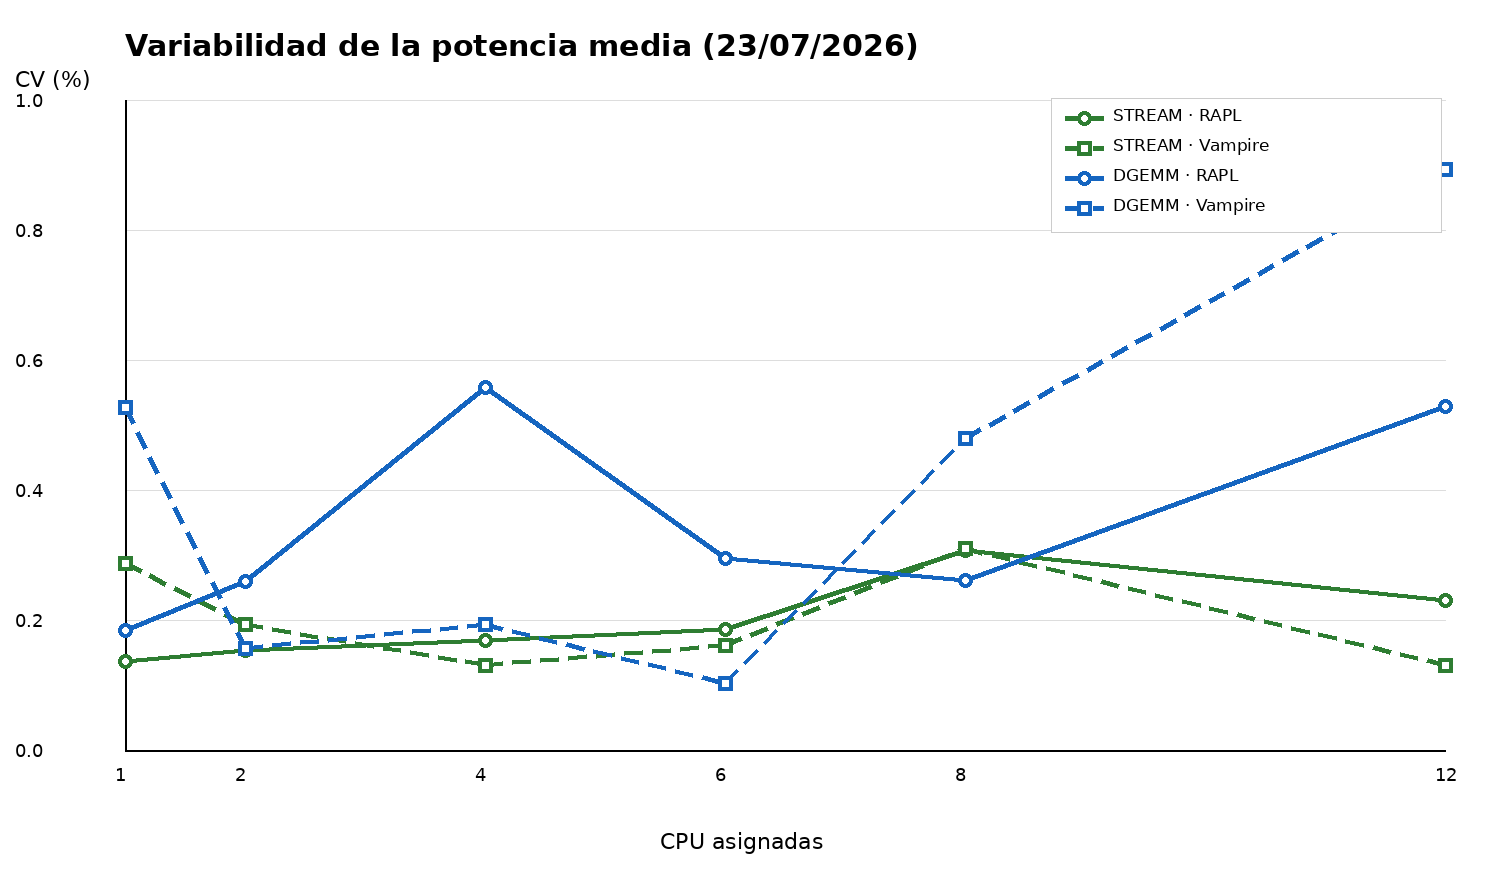
\includegraphics[width=0.94\textwidth]{imagenes/capitulo6/variabilidad_potencia.png}
    \caption{Coeficiente de variación de la potencia media RAPL y Vampire entre repeticiones.}
    \label{fig:variabilidad-potencia-cap6}
\end{figure}

\section{Resultados del programa de referencia Idle}
\label{sec:resultados-idle}

La ejecución de la prueba Idle tarda aproximadamente 120,5~s. RAPL registra 2,858~kJ, 23,703~W de potencia media y 28,323~W de potencia máxima. Vampire registra 10,926~kJ, 90,957~W de media y 93,4~W de máxima. La tabla~\ref{tab:idle-cap6} recoge estos valores.

\begin{table}[htbp]
    \centering
    \caption{Resultados de las fuentes interna y externa durante Idle.}
    \label{tab:idle-cap6}
    \begin{tabular}{lrr}
\hline
Métrica & RAPL & Vampire \\
\hline
Duración integrada (s) & 120.549 & 120.125 \\
Muestras & 104 & 24 \\
Energía (kJ) & 2.858 & 10.926 \\
Potencia media (W) & 23.703 & 90.957 \\
Potencia máxima (W) & 28.323 & 93.400 \\
\hline
\end{tabular}

\end{table}

La diferencia media de aproximadamente 67,3~W representa el consumo eléctrico observado externamente que no forma parte de los componentes leídos con RAPL, además de las diferencias propias de cada mecanismo de medida. Al existir una única ejecución Idle, este valor sirve como referencia y no se puede estimar su variabilidad.

\section{Resultados de STREAM}
\label{sec:resultados-stream}

El ancho de banda de memoria medido por STREAM pasa de ser 10,010~GB/s al ejecutar un proceso a 19,932~GB/s al ejecutar dos procesos en paralelo. Alcanza su mayor valor, 22,422~GB/s, con cuatro procesos, y después se mantiene alrededor de 22,2~GB/s cuando se ejecutan hasta doce procesos. La aceleración (speedup) es de 1,991 con el proceso p2, aumenta hasta 2,240 con el proceso p4 y se mantiene prácticamente igual, en 2,227, con el proceso p12. Esto muestra que el rendimiento mejora al principio, pero después se estabiliza..

La potencia obtenida a partir de los valores leídos por RAPL va de 74,018 W hasta 109,463~W. La potencia global calculada a partir de los valores obtenidos con Vampire van desde 156,282 W hasta 198,991~W. La energía medida con RAPL  toma los valores de 8,938 kJ a 13,555~kJ y de 18,832 kJ a 24,558~kJ cuando se obtiene a partir de las medidas con Vampire. Ambas fuentes presentan una evolución consistente respecto al aumento de los recursos asignados, sin cambios de tendencia en los valores registrados.

Las medidas asociadas a RAPL son crecientes, desde un 47,5~\% en el proceso \texttt{p1} hasta un 55,2~\% en el proceso \texttt{p12}. La diferencia entre el consumo global del sistema y las medidas internas se encuentran entre 9,89 kJ y 11,00~kJ. 

\section{Resultados de DGEMM}
\label{sec:resultados-dgemm}

El rendimiento obtenido con DGEMM aumenta de forma progresiva a medida que se incrementa el número de procesos: pasa de 0,668 GFLOP/s con un proceso a 1,378 GFLOP/s con dos, 2,406 GFLOP/s con cuatro, 2,856 GFLOP/s con seis, 3,291 GFLOP/s con ocho y 4,023 GFLOP/s con doce. Con doce procesos se alcanza una aceleración (speedup) de 6,022, lo que corresponde a una eficiencia paralela del 50,2~\%.

Al aumentar el número de procesos, ambas fuentes de medida muestran un incremento progresivo de la potencia media y de la energía consumida. En RAPL, la potencia media pasa de 74,870~W a 125,953~W, mientras que Vampire registra un aumento de 153,425~W a 221,225~W. De forma coherente, la energía acumulada crece desde 9,170 hasta 15,854~kJ en RAPL y desde 18,769 hasta 27,697~kJ en Vampire. Aunque la medida externa es superior en todos los casos, la proporción que representa RAPL respecto a Vampire aumenta del 48,9~\% al 57,2~\%. Al mismo tiempo, la diferencia absoluta entre ambas medidas también crece, pasando de 9,60 a 11,84~kJ.

Estos resultados indican que el aumento de la carga incrementa el consumo observado por ambas fuentes, pero no de forma idéntica, ya que RAPL y Vampire cubren ámbitos distintos del sistema.

La tabla~\ref{tab:resumen-activos} reúne los resultados medios de las cinco repeticiones para las dos cargas activas.

\begin{table}[htbp]
    \centering
    \caption{Rendimiento y medidas energéticas medias de STREAM y DGEMM.}
    \label{tab:resumen-activos}
    \resizebox{\textwidth}{!}{\begin{tabular}{lrrrrrrrr}
\hline
Benchmark & CPU & Rend. & Unidad & RAPL (W) & Vampire (W) & RAPL (kJ) & Vampire (kJ) & Cobertura (\%) \\
\hline
STREAM & 1 & 10.010 & GB/s & 74.02 & 156.28 & 8.94 & 18.83 & 47.5 \\
STREAM & 2 & 19.932 & GB/s & 85.18 & 170.53 & 10.30 & 20.57 & 50.1 \\
STREAM & 4 & 22.422 & GB/s & 91.92 & 178.78 & 11.15 & 21.63 & 51.5 \\
STREAM & 6 & 22.214 & GB/s & 95.40 & 182.98 & 11.64 & 22.27 & 52.3 \\
STREAM & 8 & 22.186 & GB/s & 99.91 & 188.27 & 12.28 & 23.04 & 53.3 \\
STREAM & 12 & 22.298 & GB/s & 109.46 & 198.99 & 13.56 & 24.56 & 55.2 \\
DGEMM & 1 & 0.668 & GFLOP/s & 74.87 & 153.43 & 9.17 & 18.77 & 48.9 \\
DGEMM & 2 & 1.378 & GFLOP/s & 85.88 & 166.46 & 10.58 & 20.42 & 51.8 \\
DGEMM & 4 & 2.406 & GFLOP/s & 97.91 & 180.19 & 12.11 & 22.19 & 54.6 \\
DGEMM & 6 & 2.856 & GFLOP/s & 106.09 & 192.00 & 13.12 & 23.65 & 55.5 \\
DGEMM & 8 & 3.291 & GFLOP/s & 114.12 & 203.22 & 14.20 & 25.18 & 56.4 \\
DGEMM & 12 & 4.023 & GFLOP/s & 125.95 & 221.23 & 15.85 & 27.70 & 57.2 \\
\hline
\end{tabular}
}
\end{table}

\section{Relación entre las medidas obtenidas con RAPL y Vampire}
\label{sec:resultados-vampire}

La Figura~\ref{fig:potencia-nucleos-cap6} compara la evolución de la potencia media registrada mediante RAPL y Vampire para STREAM y DGEMM al aumentar el número de CPU asignadas. Las cuatro series permiten observar tanto las diferencias entre los dos programas de referencia como la respuesta de las medidas interna y externa ante el incremento de recursos. Los valores obtenidos mediante Vampire son superiores a los registrados por RAPL debido al distinto alcance de ambas fuentes: RAPL considera los dominios \texttt{package} de los procesadores, mientras que Vampire mide el consumo eléctrico global del nodo.

\begin{figure}[htbp]
    \centering
    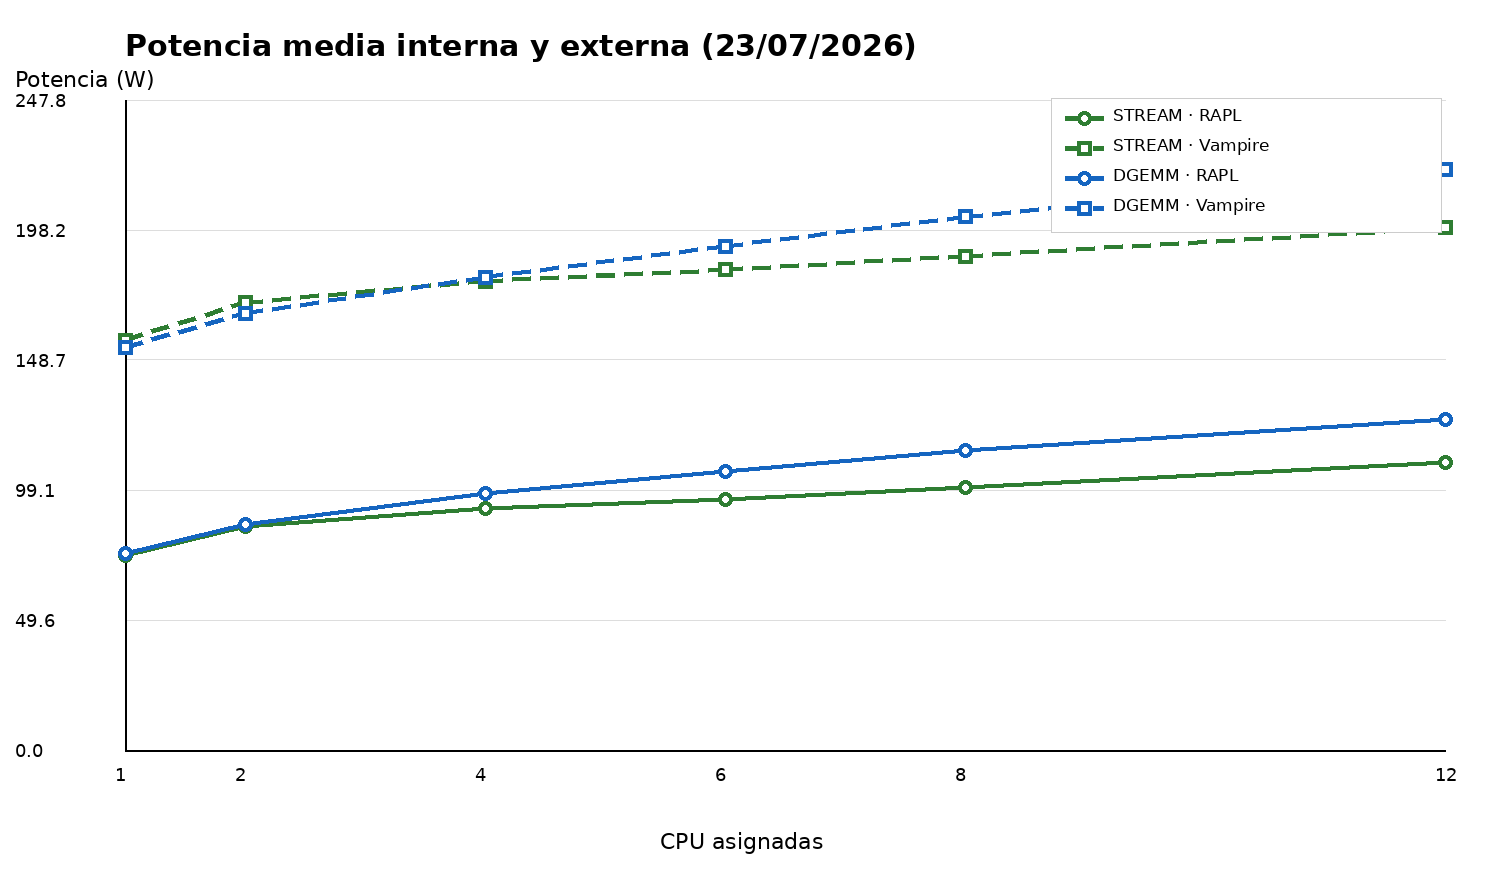
\includegraphics[width=0.94\textwidth]{imagenes/capitulo6/potencia_media_por_nucleos.png}
    \caption{Potencia media registrada mediante RAPL y Vampire para STREAM y DGEMM en función del número de CPU asignadas.}
    \label{fig:potencia-nucleos-cap6}
\end{figure}

La Figura~\ref{fig:energia-nucleos-cap6} presenta la misma comparación para la energía acumulada durante cada ejecución. Se representan las medidas de RAPL y Vampire para las seis configuraciones de STREAM y DGEMM.

\begin{figure}[htbp]
    \centering
    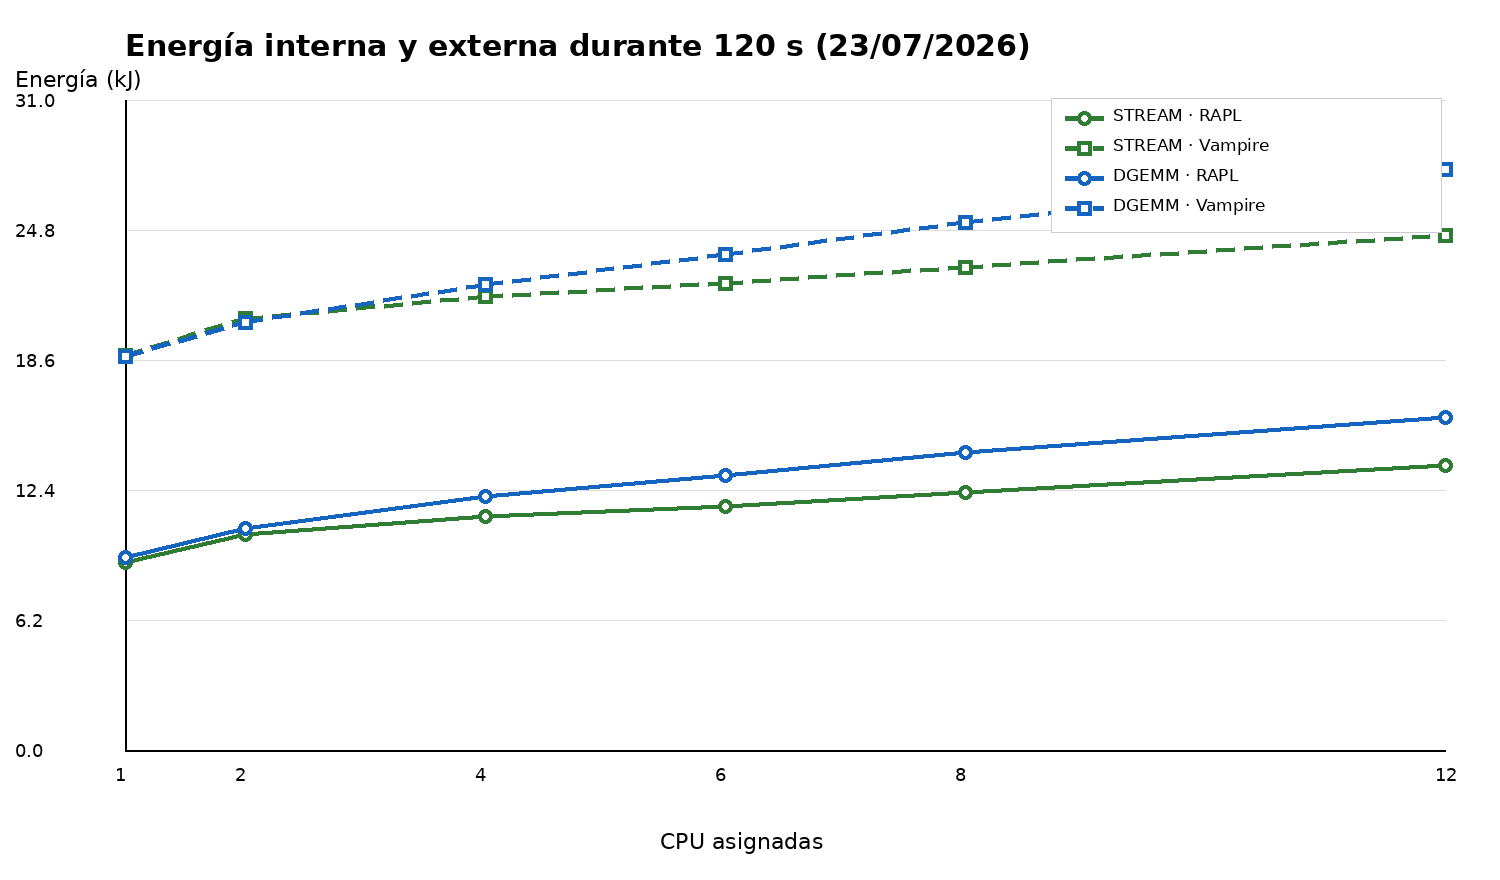
\includegraphics[width=0.94\textwidth]{imagenes/capitulo6/energia_por_nucleos.png}
    \caption{Energía registrada mediante RAPL y Vampire para STREAM y DGEMM en función del número de CPU asignadas, con una duración objetivo de 120~s por ejecución}
    \label{fig:energia-nucleos-cap6}
\end{figure}

Las cuatro series muestran un incremento de la energía al aumentar el número de CPU asignadas. La evolución es similar a la observada en la potencia media debido a que las ejecuciones tienen una duración objetivo aproximadamente constante. Vampire registra valores superiores a RAPL en todas las configuraciones, mientras que DGEMM presenta un crecimiento más acusado que STREAM al aumentar el número de procesos. Estas diferencias se interpretan considerando que ambas fuentes miden dominios energéticos distintos.

La Tabla~\ref{tab:vampire-cap6} muestra la diferencia entre la energía registrada mediante RAPL y Vampire, así como la relación porcentual entre ambas medidas. En todas las ejecuciones analizadas, Vampire registra valores superiores a RAPL, como corresponde al distinto alcance de cada fuente: RAPL considera los dominios \texttt{package} de los procesadores, mientras que Vampire mide el consumo eléctrico global del nodo. Además, las medidas externas presentan una baja variabilidad entre repeticiones y aumentan de forma coherente al incrementar la carga. Estos resultados permiten comprobar que la integración de Vampire proporciona medidas consistentes durante la campaña, aunque no permiten considerar RAPL y Vampire como instrumentos equivalentes ni constituyen una calibración de ninguno de ellos.

\begin{table}[htbp]
    \centering
    \caption{Energía consumida medida con RAPL y Vampire.}
    \label{tab:vampire-cap6}
    \resizebox{\textwidth}{!}{%
        \begin{tabular}{lrrrr}
\hline
Benchmark & CPU & Vampire--RAPL (kJ) & RAPL/Vampire (\%) & Vampire/RAPL \\
\hline
STREAM & 1 & 9.89 & 47.5 & 2.107 \\
STREAM & 2 & 10.27 & 50.1 & 1.997 \\
STREAM & 4 & 10.48 & 51.5 & 1.940 \\
STREAM & 6 & 10.63 & 52.3 & 1.913 \\
STREAM & 8 & 10.76 & 53.3 & 1.876 \\
STREAM & 12 & 11.00 & 55.2 & 1.812 \\
DGEMM & 1 & 9.60 & 48.9 & 2.047 \\
DGEMM & 2 & 9.83 & 51.8 & 1.929 \\
DGEMM & 4 & 10.08 & 54.6 & 1.833 \\
DGEMM & 6 & 10.53 & 55.5 & 1.803 \\
DGEMM & 8 & 10.98 & 56.4 & 1.773 \\
DGEMM & 12 & 11.84 & 57.2 & 1.747 \\
\hline
\end{tabular}
%
    }
\end{table}

\section{Análisis de escalabilidad}
\label{sec:analisis-escalabilidad}
A continuación se analiza cómo evoluciona el comportamiento de los programas de referencia al aumentar el número de CPU asignadas. Para ello se estudian el rendimiento, la potencia y la energía obtenidos para los distintos perfiles de ejecución, así como la eficiencia de escalado y la eficiencia energética. El objetivo es determinar hasta qué punto el incremento de recursos se traduce en una mejora efectiva del rendimiento y cómo varía, al mismo tiempo, el consumo energético.

\subsection{Rendimiento}

La figura~\ref{fig:speedup-nucleos-cap6} muestra la evolución de la aceleración (speedup) de los programas de pruebas, STREAM y DGEMM, al aumentar el número de CPUs asignadas. En el eje horizontal aparece el número de CPU asignadas y en el vertical la aceleración (speedup). La línea gris representa la escalabilidad ideal, es decir,  si se duplicaran los recursos, el rendimiento también debería duplicarse. STREAM mejora claramente al pasar de uno a dos procesos, pero a partir de 4 procesos el aumento es mucho menor y finalmente el rendimiento prácticamente se estabiliza. Esto indica que añadir más CPUs no supone una mejora significativa, probablemente porque se alcanza una limitación asociada al ancho de banda de memoria. DGEMM continúa aumentando su rendimiento conforme se incrementan las CPUs. Sin embargo, su crecimiento también está por debajo del ideal: con 12 CPUs alcanza una acelaración de aproximadamente 6, en lugar de 12. Por tanto, sigue aprovechando los recursos adicionales, aunque con una eficiencia cada vez menor. Ambos programas permanecen por debajo de la escalabilidad ideal, siendo esta diferencia especialmente acusada en STREAM. 

\begin{figure}[htbp]
    \centering
    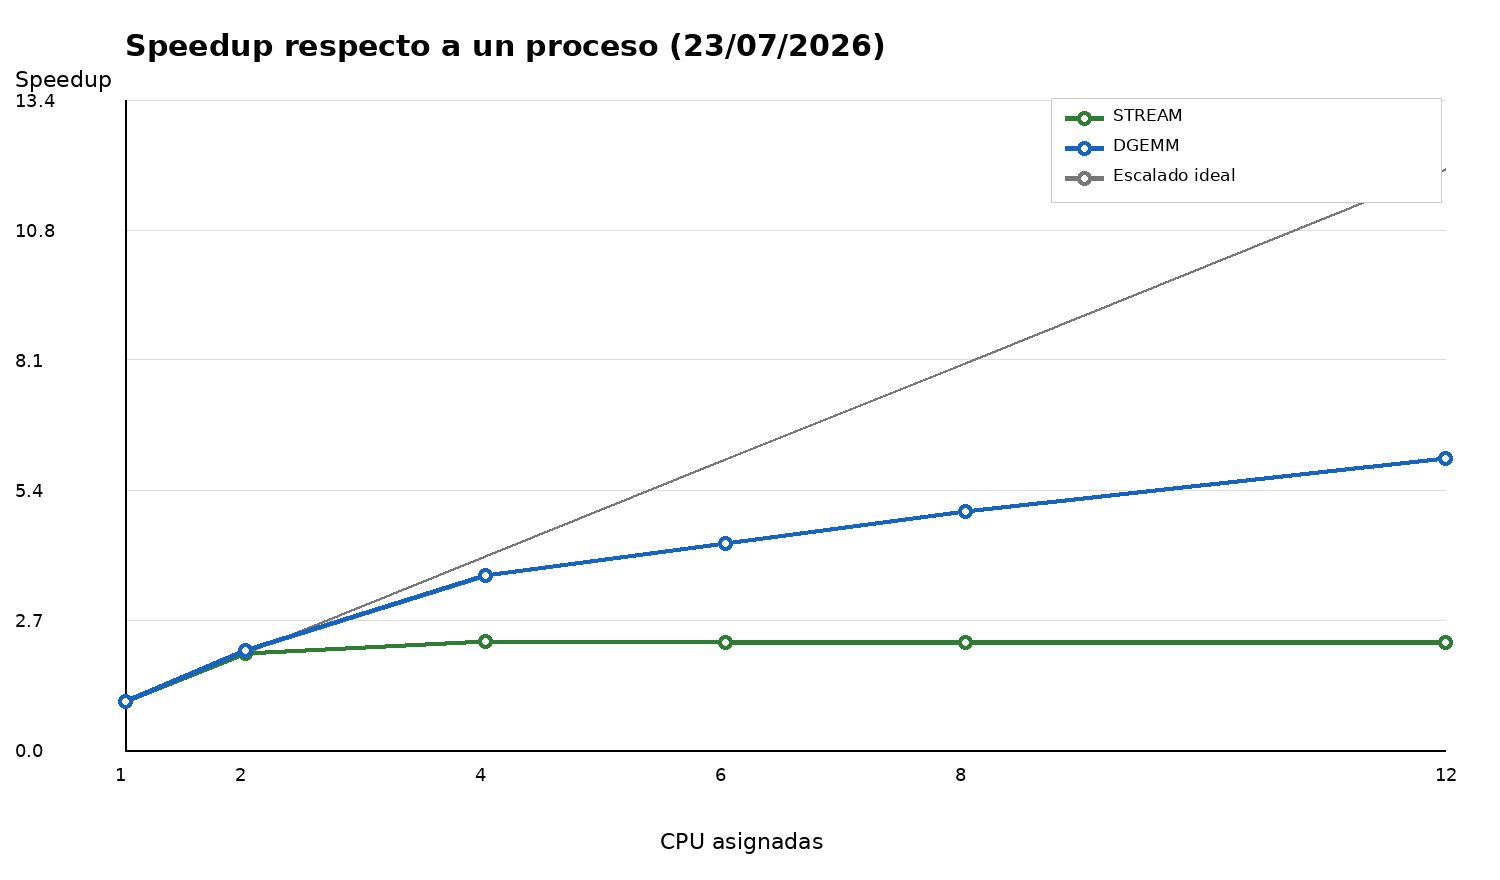
\includegraphics[width=0.92\textwidth]{imagenes/capitulo6/speedup_por_nucleos.png}
    \caption{Aceleración de STREAM y DGEMM con el número de CPUs.}
    \label{fig:speedup-nucleos-cap6}
\end{figure}

\subsection{Potencia y energía}

La figura 6.5 muestra cómo evoluciona en el tiempo la potencia medida con RAPL durante varias ejecuciones de STREAM y DGEMM, con 1 proceso (p1) y con 12 procesos (p12).

Las series temporales obtenidas con RAPL muestran un consumo de potencia estable durante la mayor parte de las ejecuciones. Con un proceso, STREAM y DGEMM se mantienen en torno a 50 W, mientras que con doce procesos la potencia aumenta hasta aproximadamente 95 W. En STREAM, aumentar de cuatro a doce procesos apenas modifica el rendimiento, pero eleva la energía obtenida con RAPL un 21,6~\% y la energía obtenida con Vampire un 13,5~\%

Además, el gráfico muestra que el número de procesos tiene mucha más influencia sobre la potencia que el tipo de programa, ya que STREAM y DGEMM presentan valores bastante similares cuando utilizan el mismo número de procesos. Sin embargo, esto no significa que tengan el mismo rendimiento: como se veía en el gráfico anterior, DGEMM aprovecha mucho mejor el aumento de procesos que STREAM. Al finalizar las ejecuciones se observa una caída brusca de la potencia, correspondiente a la finalización de la ejecución.  
\begin{figure}[htbp]
    \centering
    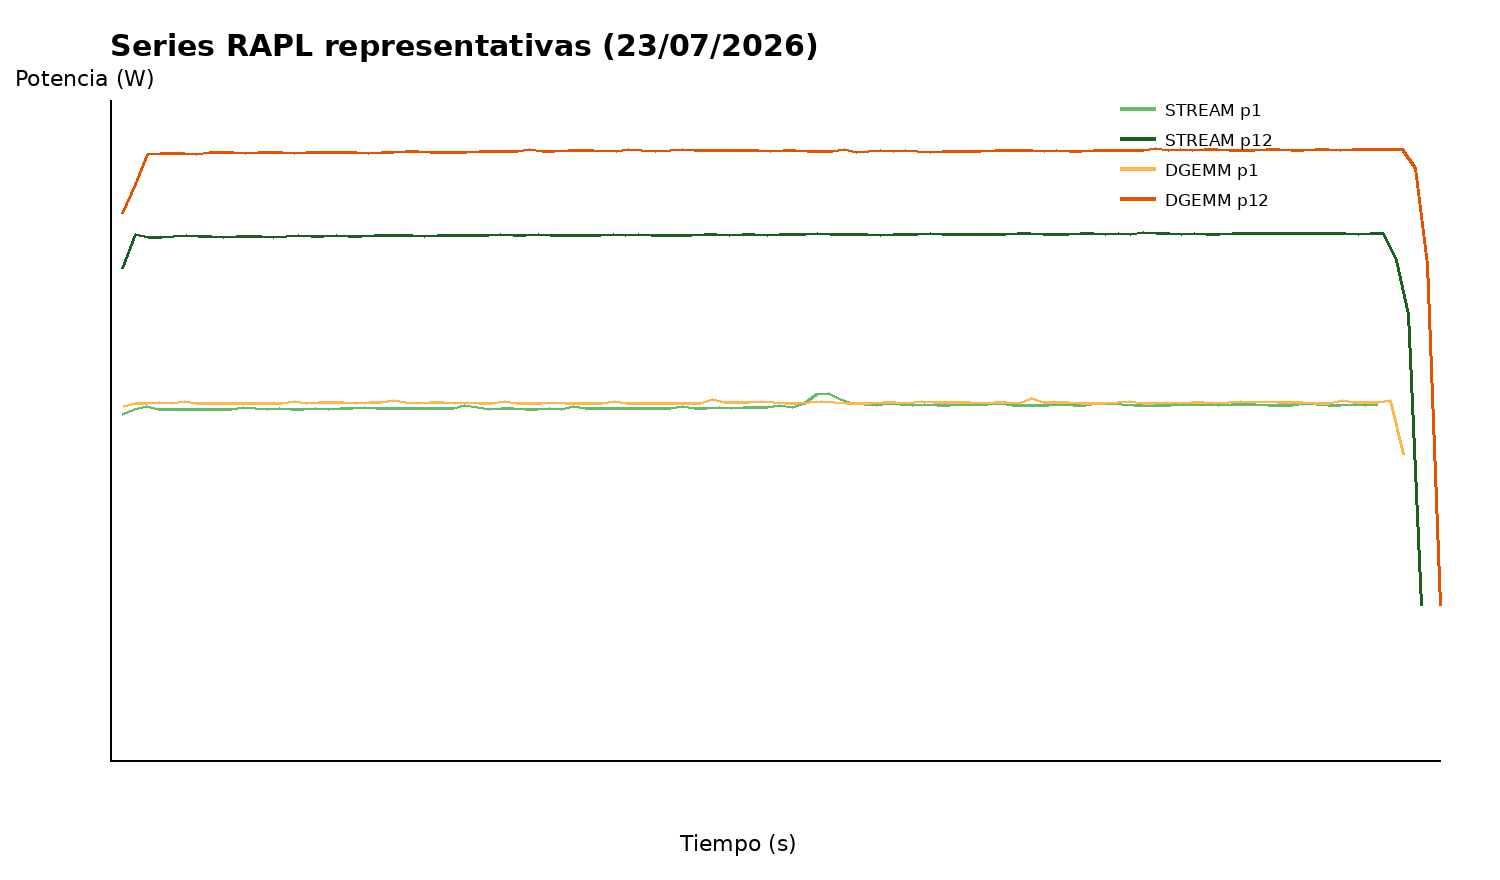
\includegraphics[width=0.94\textwidth]{imagenes/capitulo6/series_rapl_representativas.png}
    \caption{Evolución temporal de la potencia medida con RAPL  para STREAM y DGEMM.}
    \label{fig:series-rapl-cap6}
\end{figure}

\subsection{Eficiencia energética}

La eficiencia energética mide el rendimiento que se obtiene por cada unidad de energía o potencia consumida. En este trabajo se calcula dividiendo el trabajo total realizado por la energía consumida durante la ejecución para STREAM y se expresa en bytes/j, mientras que para DGEMM se expresa en operaciones/J

La evolución de la eficiencia energética muestra comportamientos claramente diferentes para STREAM y DGEMM. En ambos casos, el perfil de un proceso se utiliza como referencia, por lo que un valor superior a 1 indica que la cantidad de trabajo realizada por cada julio consumido ha aumentado respecto a dicha configuración.

En STREAM, la eficiencia energética mejora al pasar de uno a dos y cuatro procesos, alcanzando su valor máximo en el perfil de cuatro procesos. A partir de este punto, la tendencia se invierte y la eficiencia disminuye progresivamente al utilizar seis, ocho y doce procesos. Este comportamiento está relacionado con la evolución del rendimiento observada anteriormente: STREAM aumenta considerablemente su rendimiento hasta cuatro procesos, pero a partir de ese perfil permanece prácticamente estable. Sin embargo, la energía consumida continúa aumentando al incorporar más recursos. En consecuencia, los perfiles superiores a cuatro procesos consumen más energía sin producir un incremento proporcional de la cantidad de datos procesados.

DGEMM presenta un comportamiento diferente. Su eficiencia energética aumenta de forma sostenida al incrementar el número de procesos y alcanza su valor máximo con doce. En este caso, el aumento del consumo energético producido al utilizar más recursos se acompaña de un crecimiento suficiente del rendimiento, por lo que la cantidad de operaciones realizadas por julio continúa mejorando. Esto indica que, dentro del rango analizado, DGEMM aprovecha de forma más efectiva el incremento de los recursos de cálculo que STREAM.

Estos resultados muestran que la configuración energéticamente más eficiente depende del tipo de carga. En STREAM, aumentar el número de procesos más allá de cuatro deja de resultar favorable desde el punto de vista de la eficiencia energética, mientras que DGEMM continúa beneficiándose del aumento de recursos hasta el máximo estudiado. Por tanto, asignar un mayor número de CPU no garantiza por sí mismo una utilización más eficiente de la energía: es necesario considerar conjuntamente el aumento del rendimiento y el incremento del consumo producido por cada configuración.

La Figura~\ref{fig:eficiencia-energetica-cap6} permite observar esta diferencia de forma directa. Mientras que STREAM presenta un máximo seguido de una disminución progresiva, DGEMM mantiene una tendencia creciente. Esta diferencia refuerza la idea de que no existe un único perfil óptimo para todas las cargas y que la selección de recursos puede variar en función del objetivo perseguido, ya sea maximizar el rendimiento, limitar el consumo o aumentar la cantidad de trabajo realizada por unidad de energía.

\begin{figure}[htbp]
    \centering
    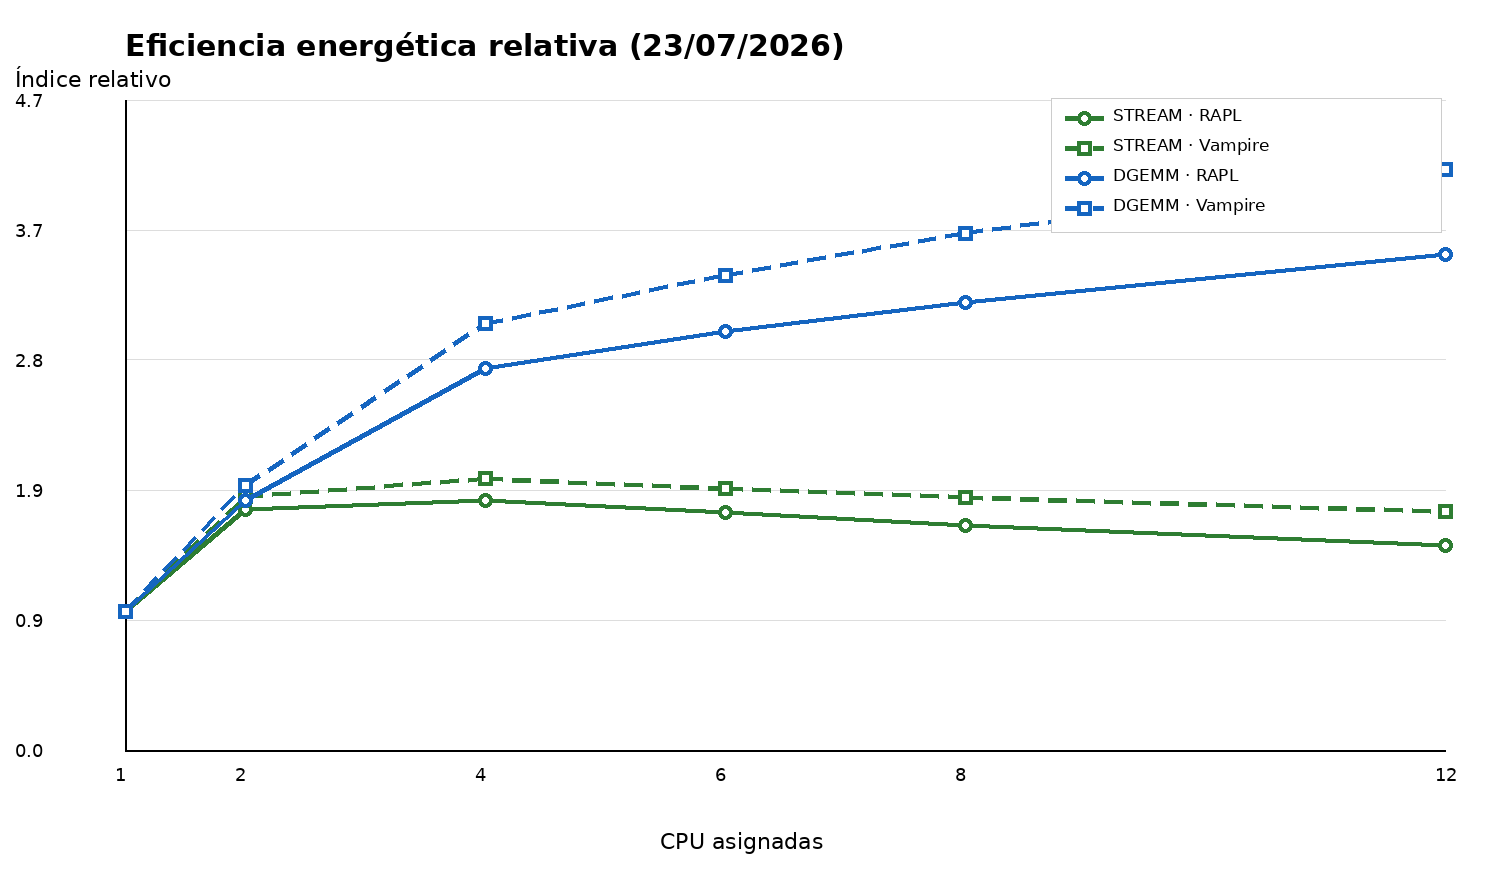
\includegraphics[width=0.92\textwidth]{imagenes/capitulo6/eficiencia_energetica_relativa.png}
    \caption{Evolución de la eficiencia energética relativa con el número de procesos.}
    \label{fig:eficiencia-energetica-cap6}
\end{figure}

La tabla~\ref{tab:escalabilidad-cap6} compara cómo evolucionan la aceleración, la eficiencia paralela y la eficiencia energética de STREAM y DGEMM al aumentar el número de CPU asignadas.

\begin{table}[htbp]
    \centering
    \caption{Indicadores de escalabilidad y eficiencia energética para STREAM y DGEMM.}
    \label{tab:escalabilidad-cap6}
    \resizebox{\textwidth}{!}{\begin{tabular}{lrrrrr}
\hline
Benchmark & CPU & Speedup & Eficiencia paralela (\%) & Efic. RAPL & Efic. Vampire \\
\hline
STREAM & 1 & 1.000 & 100.0 & 1.000 & 1.000 \\
STREAM & 2 & 1.991 & 99.6 & 1.728 & 1.823 \\
STREAM & 4 & 2.240 & 56.0 & 1.797 & 1.951 \\
STREAM & 6 & 2.219 & 37.0 & 1.706 & 1.879 \\
STREAM & 8 & 2.216 & 27.7 & 1.618 & 1.817 \\
STREAM & 12 & 2.227 & 18.6 & 1.474 & 1.715 \\
DGEMM & 1 & 1.000 & 100.0 & 1.000 & 1.000 \\
DGEMM & 2 & 2.062 & 103.1 & 1.792 & 1.901 \\
DGEMM & 4 & 3.601 & 90.0 & 2.745 & 3.067 \\
DGEMM & 6 & 4.275 & 71.3 & 3.009 & 3.417 \\
DGEMM & 8 & 4.926 & 61.6 & 3.222 & 3.720 \\
DGEMM & 12 & 6.022 & 50.2 & 3.565 & 4.177 \\
\hline
\end{tabular}
}
\end{table}

\section{Análisis estadístico}
\label{sec:estadistica-cap6}
En los siguientes subapartados se detalla el análisis estadístico llevado a cabo con los datos obtenidos.  Para ello se estudia, en primer lugar, la variabilidad entre repeticiones de una misma configuración con el objetivo de comprobar la estabilidad de las medidas. A continuación, se analizan las relaciones entre las principales métricas de rendimiento y consumo energético mediante medidas de correlación. Finalmente, se comparan los comportamientos observados entre los distintos programas de referencia y perfiles de ejecución, tratando de identificar tendencias consistentes y diferencias relevantes entre configuraciones.

\subsection{Estadística descriptiva y variabilidad}

Las medias y los coeficientes de variación muestran que energía y potencia son más estables que el rendimiento DGEMM. La mayor dispersión energética es 0,65~\% para RAPL y 1,04~\% para Vampire. La potencia media no supera 0,57~\% en RAPL ni 0,91~\% en Vampire. Estas cifras permiten distinguir los perfiles sin que la variación entre repeticiones domine las tendencias.

\subsection{Matriz de correlación}

Con el objetivo de estudiar si existe una relación entre las principales variables registradas durante la campaña, se ha calculado una matriz de correlación. Este tipo de matriz permite comparar varias variables entre sí y resumir, en una única representación, hasta qué punto dos magnitudes tienden a variar de forma conjunta.

Para cuantificar esta relación se utiliza el coeficiente de correlación de Pearson. Este coeficiente toma valores comprendidos entre \(-1\) y \(1\). Un valor próximo a \(1\) indica que, cuando una variable aumenta, la otra tiende también a aumentar. Un valor próximo a \(-1\) indica una evolución en sentido contrario, mientras que un valor cercano a \(0\) indica que no existe una relación lineal clara entre ambas variables. La correlación mide, por tanto, el grado de asociación lineal entre dos magnitudes, pero no permite afirmar por sí sola que una sea la causa de la otra.

La matriz de correlación se ha utilizado en este trabajo porque permite comprobar de forma sencilla si los cambios introducidos en las configuraciones experimentales se reflejan de manera consistente en las métricas de consumo. En particular, resulta de interés estudiar la relación entre el número de CPU asignadas y la energía registrada, así como comprobar si las medidas obtenidas mediante RAPL y Vampire presentan una evolución similar a lo largo de las distintas ejecuciones.

Para este análisis se consideran las 60 ejecuciones correspondientes a las cargas activas, STREAM y DGEMM. La ejecución Idle no se incluye, ya que constituye una única referencia basal y no forma parte de los perfiles repetidos utilizados para estudiar la variación con el número de CPU.

La Figura~\ref{fig:matriz-correlacion-cap6} muestra los valores obtenidos. El número de CPU asignadas presenta una correlación de \(0{,}911\) con la energía registrada mediante RAPL y de \(0{,}928\) con la energía medida por Vampire. Ambos valores son elevados y positivos, lo que indica que, dentro de las configuraciones analizadas, el aumento del número de CPU está asociado generalmente a un incremento de la energía consumida.

La correlación más elevada se observa entre las energías registradas mediante RAPL y Vampire, con un valor de \(r=0{,}995\). Este resultado indica que ambas magnitudes siguen una evolución lineal muy similar entre las diferentes ejecuciones: cuando aumenta la energía registrada mediante RAPL, también tiende a aumentar la energía medida externamente por Vampire.

Sin embargo, este resultado no significa que ambas herramientas estén midiendo la misma parte del sistema. RAPL registra la energía correspondiente a los dominios \texttt{package} de los procesadores, mientras que Vampire mide el consumo eléctrico global del nodo. Por tanto, la elevada correlación debe interpretarse como una similitud en la evolución de ambas medidas ante los cambios de carga y de recursos, y no como una equivalencia entre los dos sistemas de medición.

\begin{figure}[H]
    \centering
    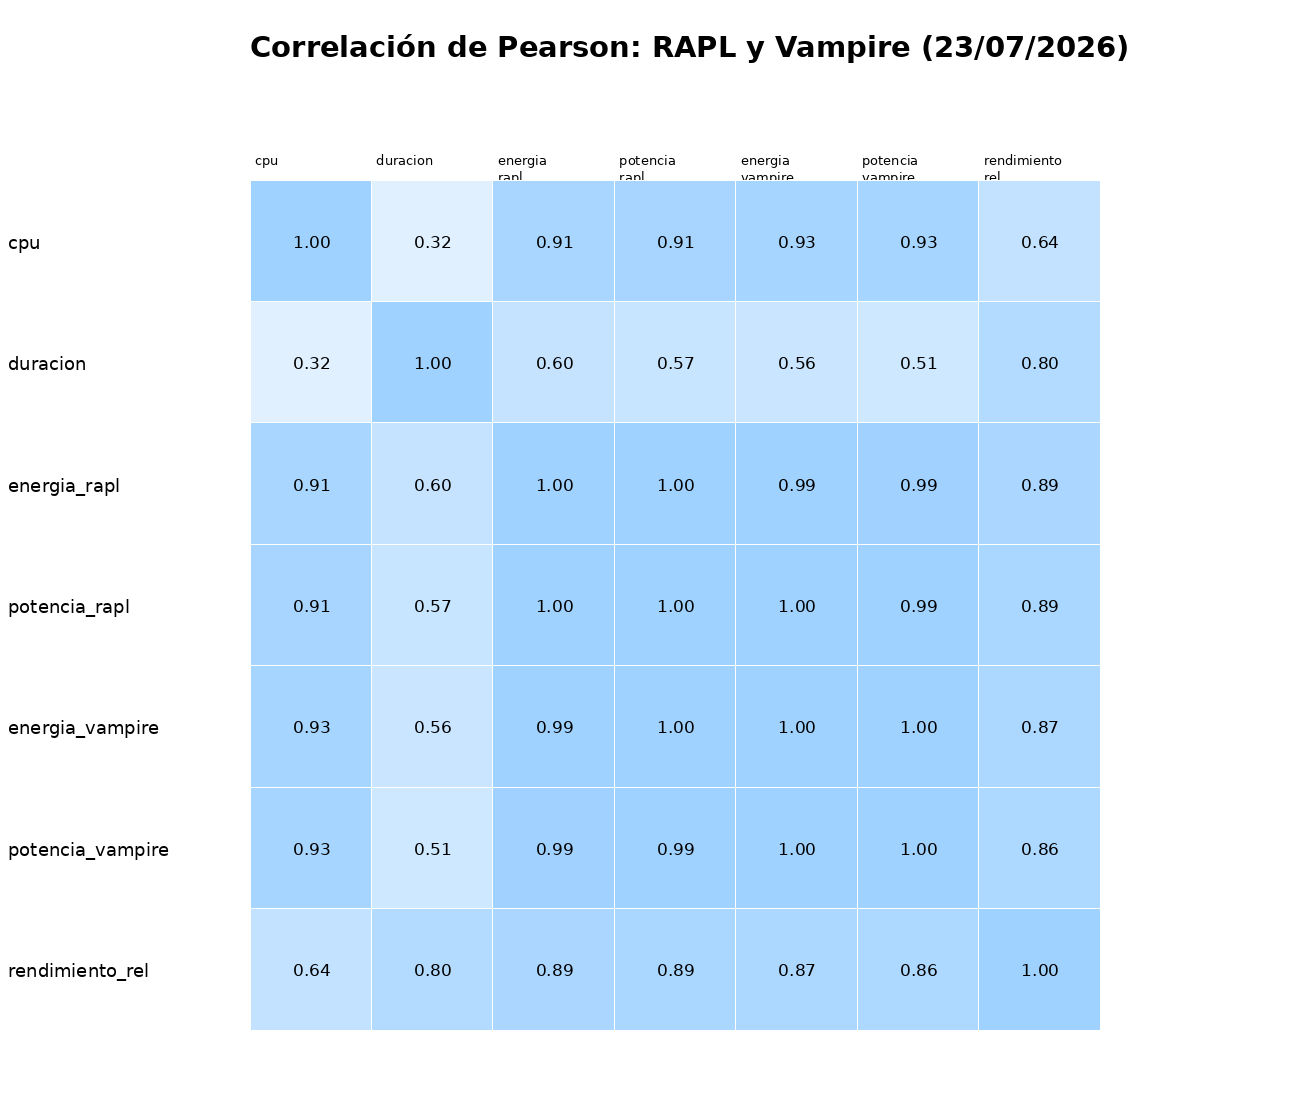
\includegraphics[width=0.90\textwidth]{imagenes/capitulo6/matriz_correlacion.png}
    \caption{Matriz de correlación de Pearson para métricas internas, externas y de rendimiento.}
    \label{fig:matriz-correlacion-cap6}
\end{figure}

La correlación entre energía y potencia es parcialmente estructural porque las duraciones son próximas. Del mismo modo, el rendimiento relativo deriva del trabajo y del tiempo. La matriz se utiliza para controlar la coherencia y para detectar la existencia de variables redundantes, no para demostrar causalidad.

\subsection{Selección e interpretación de métricas}

Para caracterizar cada ejecución se han seleccionado métricas relacionadas con tres aspectos principales: el tiempo de ejecución, el rendimiento obtenido y el consumo energético. Además, se conservan algunas variables auxiliares destinadas a comprobar la calidad de las medidas. La elección de estas métricas permite analizar no solo cuánto consume una configuración, sino también cuánto trabajo realiza y cómo evoluciona su comportamiento al aumentar los recursos asignados.

La \textbf{duración} representa el tiempo durante el que se ejecuta el programa de referencia. En STREAM y DGEMM se utiliza una ventana objetivo de aproximadamente 120~s, aunque se registra el tiempo real de cada ejecución. Esta métrica permite comprobar que las distintas pruebas se han desarrollado durante intervalos comparables y sirve también para calcular las tasas de rendimiento.

El \textbf{rendimiento} expresa la cantidad de trabajo realizada por unidad de tiempo. Su definición depende del programa de referencia. En STREAM se calcula a partir de la cantidad total de datos procesados por todos los procesos y se expresa en GB/s. En DGEMM se utiliza el número de operaciones en coma flotante realizadas por unidad de tiempo y se expresa en GFLOP/s. Para obtener el rendimiento agregado se suma el trabajo realizado por todos los procesos y se divide entre la mayor duración registrada entre ellos, ya que los procesos se ejecutan de forma concurrente.

La \textbf{energía} indica la cantidad total de energía consumida durante la ventana analizada. En RAPL se obtiene sumando los incrementos de energía calculados entre lecturas consecutivas de los contadores \texttt{package}. En Vampire se calcula a partir de las muestras de potencia registradas durante la ejecución, integrándolas sobre el intervalo temporal correspondiente al programa de referencia. La energía se expresa en julios o kilojulios y permite estudiar cómo aumenta el consumo total al modificar el número de recursos utilizados.

La \textbf{potencia media} representa la velocidad media a la que se consume energía durante una ejecución y se expresa en vatios. En RAPL se obtiene a partir de la energía consumida entre muestras consecutivas y del tiempo transcurrido entre ellas. En Vampire se calcula a partir de las muestras de potencia correspondientes a la misma ventana temporal. Esta métrica permite comparar la intensidad del consumo entre configuraciones sin depender únicamente de la energía total acumulada.

La \textbf{potencia máxima} corresponde al mayor valor de potencia observado durante una ejecución. Su inclusión permite detectar los niveles máximos alcanzados durante las cargas, aunque debe interpretarse con precaución. RAPL y Vampire utilizan intervalos de muestreo diferentes, por lo que un sistema con mayor frecuencia de adquisición tiene más posibilidades de registrar variaciones breves de potencia. Por este motivo, la potencia máxima se utiliza como información complementaria y no para realizar una comparación directa muestra a muestra entre ambas fuentes.

También se calcula la \textbf{diferencia de energía entre Vampire y RAPL}, definida como:

\[
\Delta E_{\mathrm{ext-int}} =
E_{\mathrm{Vampire}} - E_{\mathrm{RAPL}}.
\]

donde \(E_{\mathrm{Vampire}}\) es la energía medida externamente para el nodo completo y \(E_{\mathrm{RAPL}}\) la energía registrada en los dominios \texttt{package} seleccionados. Esta diferencia permite cuantificar cuánto mayor es la medida externa respecto a la interna. No debe interpretarse como el consumo exacto del resto de componentes del nodo, ya que ambas herramientas presentan alcances de medida diferentes y la diferencia no permite realizar una descomposición energética por componentes.

Para estudiar la relación entre ambas fuentes se calcula además la \textbf{cobertura RAPL}, definida como:

\[
C_{\mathrm{RAPL}} =
100\,
\frac{E_{\mathrm{RAPL}}}
     {E_{\mathrm{Vampire}}}.
\]

Esta métrica expresa qué porcentaje de la energía registrada externamente por Vampire representa la energía medida mediante los dominios RAPL seleccionados. Por ejemplo, una cobertura del 50~\% indica que la energía registrada mediante RAPL equivale aproximadamente a la mitad de la energía medida externamente durante esa ejecución. Este porcentaje no debe interpretarse como la fracción exacta del consumo del nodo atribuible a la CPU, sino como una relación entre los alcances de las dos fuentes de medida utilizadas en el trabajo.

Por último, el \textbf{número de muestras} y el \textbf{estado de la captura} se conservan como indicadores de calidad. El número de muestras permite comprobar que la ejecución contiene suficientes observaciones para cubrir el intervalo analizado, mientras que el estado de captura indica si el proceso de adquisición finalizó correctamente. Estas variables no se utilizan como resultados energéticos principales, pero permiten detectar ejecuciones incompletas o potencialmente inválidas antes de incorporarlas al análisis.

En conjunto, estas métricas permiten estudiar cada configuración desde distintas perspectivas. La duración y el rendimiento describen el trabajo realizado, la energía y la potencia caracterizan el consumo, la diferencia y la cobertura permiten analizar la relación entre las medidas internas y externas, y los indicadores de calidad ayudan a asegurar que los datos utilizados en el análisis proceden de ejecuciones correctamente registradas.

\section{Evaluación global del sistema}
\label{sec:evaluacion-global-cap6}

En los siguientes apartados se realiza una valoración conjunta del funcionamiento del sistema a partir de los resultados obtenidos en la campaña final. Para ello se consideran tanto la calidad y consistencia de las medidas como la capacidad de la plataforma para distinguir el comportamiento de las distintas cargas y configuraciones. El objetivo es comprobar si la infraestructura desarrollada cumple de forma adecuada su función como herramienta de medición, análisis y comparación del consumo energético en HPMoon.

\subsection{Funcionalidad}

De los resultados obtenidos tras las ejecuciones se puede deducir que el sistema es capaz de completar y coordinar las 61 ejecuciones mediante SLURM, obtener medidas energéticas de los dominios \texttt{package} de los procesadores mediante RAPL y del consumo eléctrico global del nodo mediante Vampire, procesar estos datos, conservar los resultados y publicar las métricas asociadas a un mismo identificador de ejecución (\texttt{run\_id}). Además, el sistema organiza estas tareas en etapas diferenciadas: la configuración define las condiciones de la prueba, la ejecución lanza el programa de referencia, la adquisición recoge las medidas, el almacenamiento conserva los resultados, la publicación envía las métricas al sistema de monitorización y el análisis procesa posteriormente los datos obtenidos. Esta organización facilita revisar o modificar cada etapa sin alterar necesariamente el resto del flujo.

\subsection{Coherencia}

En este trabajo, la coherencia de los resultados se entiende como la consistencia entre los datos almacenados, los valores recalculados a partir de las muestras originales y la evolución observada al modificar las condiciones de ejecución. Evaluar esta coherencia es importante porque permite comprobar que el sistema de medida y procesamiento no introduce discrepancias internas y que las métricas obtenidas responden de forma estable a los cambios de carga.

Para ello se han realizado varias comprobaciones. En primer lugar, los valores agregados de energía y potencia se han recalculado a partir de los archivos CSV originales y se ha verificado que coinciden con los resultados almacenados. En segundo lugar, se ha comprobado que tanto las medidas obtenidas mediante RAPL como las registradas por Vampire presentan una evolución consistente al aumentar la carga y una baja dispersión entre repeticiones equivalentes. Finalmente, la relación entre ambas medidas se interpreta teniendo en cuenta su distinto alcance: RAPL registra la energía asociada a los dominios \texttt{package} de los procesadores, mientras que Vampire mide el consumo eléctrico global del nodo.

\subsection{Repetibilidad y utilidad}

La repetibilidad se evalúa mediante la realización de varias ejecuciones bajo una misma configuración. Su análisis permite comprobar hasta qué punto los resultados se mantienen estables cuando se repite una prueba en condiciones equivalentes y detectar posibles ejecuciones anómalas. Para las configuraciones activas de STREAM y DGEMM se realizaron cinco repeticiones por perfil, como compromiso entre disponer de varias observaciones para estimar la variabilidad y mantener una duración asumible de la campaña. A partir de estas repeticiones se calcularon medidas de dispersión, cuyos resultados muestran una variabilidad reducida en las principales magnitudes energéticas.

También se evalúa la capacidad del sistema para distinguir diferentes comportamientos de carga. Los programas utilizados representan situaciones distintas: Idle sirve como referencia de baja actividad, STREAM genera una carga orientada principalmente al subsistema de memoria y DGEMM una carga intensiva de cálculo. Los resultados permiten observar diferencias entre ambos programas al aumentar los recursos asignados. STREAM alcanza una zona en la que añadir más procesos apenas incrementa el rendimiento, mientras que DGEMM continúa mejorando dentro del rango estudiado.

Finalmente, la combinación de las métricas de rendimiento y energía permite estudiar si el aumento de los recursos asignados produce una mejora proporcional del trabajo realizado. Este análisis se realiza directamente sobre los datos almacenados de cada ejecución, mientras que los paneles de Grafana se utilizan como herramienta complementaria de visualización y supervisión.

\subsection{Alcance de la evaluación}
\label{sec:alcance-cap6}

Los resultados presentados en este capítulo deben interpretarse dentro de las condiciones concretas en las que se ha realizado la campaña experimental. La evaluación se ha llevado a cabo sobre un único nodo de cómputo de HPMoon, \texttt{compute-0-4}, utilizando tres programas de referencia y seis perfiles de ejecución para las cargas activas. STREAM y DGEMM se ejecutaron durante una ventana objetivo de 120~s y con cinco repeticiones por perfil, mientras que Idle se utilizó como referencia basal mediante una única ejecución.

Esta configuración se eligió con el objetivo de mantener un experimento suficientemente controlado y asumible en duración, evitando introducir simultáneamente un número elevado de variables. Por este motivo, el estudio se centra principalmente en analizar cómo varían el rendimiento y el consumo energético al modificar el número de procesos asignados a cada carga.

Otros factores que pueden influir en el comportamiento del sistema no se estudian de forma específica en esta campaña. Entre ellos se encuentran la distribución de procesos y memoria dentro de la arquitectura NUMA, el uso de SMT, la afinidad física exacta sobre los núcleos, la frecuencia efectiva del procesador, la temperatura y la actividad de fondo del sistema. Aunque estos factores pueden afectar a las medidas, incorporarlos como variables experimentales habría ampliado considerablemente el número de configuraciones necesarias y dificultado la interpretación de los resultados obtenidos.

El uso de un único nodo también limita la generalización de las conclusiones. Los resultados describen el comportamiento observado en la configuración hardware evaluada y no deben extrapolarse directamente a otros nodos, procesadores o arquitecturas del clúster. Del mismo modo, los programas utilizados representan tres tipos concretos de carga y no pretenden reproducir toda la diversidad de aplicaciones que pueden ejecutarse en un entorno HPC.

Por último, las medidas obtenidas mediante RAPL y Vampire corresponden a ámbitos diferentes del sistema. RAPL registra la energía asociada a los dominios \texttt{package} de los procesadores, mientras que Vampire mide el consumo eléctrico global del nodo. Por este motivo, sus valores se analizan de forma complementaria y no como dos medidas equivalentes de una misma magnitud.

Estas limitaciones no invalidan los resultados obtenidos, sino que delimitan el alcance de las conclusiones que pueden extraerse de la campaña. La discusión global de estos resultados, junto con las posibles ampliaciones destinadas a abordar estas limitaciones, se desarrolla en el capítulo~\ref{chap:conclusiones}.

\subsection{Síntesis de los resultados}
\label{sec:sintesis-cap6}

La campaña realizada permite comprobar que la infraestructura desarrollada es capaz de ejecutar de forma automatizada las distintas configuraciones experimentales, conservar las medidas y metadatos asociados y generar resultados trazables y repetibles dentro de las condiciones estudiadas. Los datos obtenidos permiten distinguir el comportamiento de las cargas estudiadas y muestran diferencias claras en la evolución del rendimiento y del consumo al aumentar los recursos asignados.

La interpretación de estos resultados, sus implicaciones dentro del objetivo general del trabajo y las líneas de continuación que pueden plantearse a partir de las limitaciones identificadas se desarrollan en el capítulo~\ref{chap:conclusiones}.
